% Dies ist ein Beispiel-Tex-File f\"{u}r eine wissenschaftliche Arbeit
% Es kann nach Belieben ver\"{a}ndert werden
% Die Präambel ist größtenteils ausgelagert
% Details zu den Paketen sind den entsprechenden Dokus zu entnehmen
% Insbesondere die KOMA-Skript-Doku sollte jeder mal angeschaut haben
% Erstellt von K. Holste f\"{u}r den PTRA-Studiengang

% Festlegung der Dokumentklasse
\documentclass[fontsize=11pt,%
twoside,% oneside als Alternative m\"{o}glich
BCOR          = 8mm, % bei Bedarf anzupassen
DIV           = 11,  % kann nach Belieben geändert werden
titlepage     = off,%
index=totoc,%
xcolor        = pdftex,%
dvipsnames,%
%bibliography  = totoc,%
%bibliography = numbered,% bei Bedarf einschalten
listof        = notnumbered]{scrreprt}



\newif\ifdesignEins
\newif\ifdesignZwei
\newif\ifdesignDrei
\newif\ifjournalabbrev % variablendeklaration.tex wird benötigt (für verschiedene Layouts der Kapitelseite)

% Layout der Kapitelseite kann hier geändert werden
% werden alle drei Optionen ausgeklammert (mit %), wird KOMA-Default verwendet:

%\designEinstrue
%\designZweitrue
\designDreitrue

% Hier geht es um abgekürzte Journal-Namen
% True = Journalnamen werden abgekürzt, sofern Abkürzungsfeld vorhanden (shortjournal)
% False = keine Abkürzung (es reicht, die folgende Zeile auszukommentieren)
\journalabbrevtrue

% Einbindung von wichigten Paketen
\usepackage[headsepline=on, automark]{scrlayer-scrpage}
\usepackage[english, main=ngerman]{babel}  % Assuming you're using both German and English
\usepackage[utf8]{inputenc}
\usepackage[T1]{fontenc}
\usepackage{lmodern}
%\usepackage{fourier} % Adobe Utopia Font
\usepackage{microtype}
%\microtypesetup{expansion=false} % bei Verwendung von fourier eventuell notwendig
\usepackage{scrdate}
\usepackage{scrtime}
\usepackage{lastpage}
\usepackage{upgreek}
\usepackage[svgnames]{xcolor}
\usepackage{blindtext} % Erzeugt Blindtext. Nur f\"{u}r Testlauf dieses Dokuments wichtig.
\usepackage{graphicx}
\usepackage{siunitx}
\usepackage{booktabs}
\usepackage{longtable}
\usepackage{threeparttable}
\usepackage{typearea}
\usepackage{tikz}
\usepackage{tikzpagenodes}
\usepackage{epigraph}
\usepackage{ellipsis}
\usepackage{soul}
\usepackage[nohyperlinks]{acronym}
\usepackage[autostyle,german=guillemets]{csquotes}
\usepackage[defaultlines = 4, all]{nowidow}
\clubpenalty = 9999
\widowpenalty = 9999
\displaywidowpenalty = 9999
\usepackage{eurosym}

% Die AMS-Mathe-Pakete
\usepackage{amsmath}
\usepackage{amsthm}
\usepackage{amsfonts}
%%%%%%%%%%%%%%%%%%%%%

\usepackage{setspace}
\usepackage{hyperref} % immer als letztes Paket laden
% Hintergrundvariablen des PDFs
\hypersetup{pdfauthor={Martina Musterfrau},
            pdftitle={Abschlussarbeit},
            pdfsubject={Abschlussarbeit},
            pdfkeywords={Abschlussarbeit PTRA},
            pdfproducer={Latex with hyperref},
            pdfcreator={pdflatex, MikTeX, WinEDT oder andere}
            }


% Marcel packages
\usepackage{float}  % Include the float package for [H] float positioning
% Redefine "Kapitel" to "Chapter"
\addto\captionsngerman{
  \renewcommand{\chaptername}{Chapter}
}
% Redefine the figure caption label from "Abbildung" to "Figure"
\addto\captionsngerman{
  \renewcommand{\figurename}{Figure}
}


% Farbdefinitionen
\definecolor{jluhellblau}{RGB}{220, 230, 235}
\definecolor{pantoneblack}{RGB}{0,0,0}
\definecolor{jlugrau}{RGB}{83, 96, 107}
\definecolor{jlublau}{RGB}{0, 105, 179}
\definecolor{chaptergrey}{rgb}{0.7,0.7,0.7}
\definecolor{thmgreen}{RGB}{128,186,36}
\definecolor{thmgrau}{RGB}{74,92,102}
\definecolor{thmblau}{RGB}{0,59,209}
\definecolor{thmbhellblau}{RGB}{64,255,237}



% Kopf- und Fu{\ss}zeilenlayout
\clearpairofpagestyles
\automark[chapter]{chapter}
\automark*[section]{}
\ihead{}
\ohead{\headmark}
\ifoot{Erstellt am \ISOToday T\thistime} % f\"{u}r finales Dokument auskommentieren
%\ifoot{} % f\"{u}r finales Dokument aktivieren
\ofoot{\,\pagemark\ von \pageref*{LastPage}}
\chead{}
\cfoot[]{}

% Fu{\ss}notenmarker fett
\deffootnote{1em}{1em}{\bfseries\thefootnotemark\ }

% Formatierung Tabellen- und Abbildungsbeschriftung
\setcapindent{0pt} % keine Einr\"{u}ckung der Caption
\renewcommand{\floatpagefraction}{1.0}
\addtokomafont{caption}{\footnotesize}
\setkomafont{captionlabel}{\bfseries\sffamily}

% Literaturverzeichnis mit BibLaTeX
\usepackage[backend = biber, style=numeric-comp, sorting = none, giveninits = true]{biblatex}
\ifjournalabbrev
\usepackage{biblatex-shortfields}
\else\fi

\DefineBibliographyStrings{ngerman}{andothers = {{et\,al\adddot}},}
\addbibresource{references.bib}




% Es ist im Literaturverzeichnis unn\"{o}tig, DOI, URL und eprint gleichzeitig zu zeigen. Dieser Abschnitt macht eine
% Fallunterscheidung. Ist die DOI vorhanden, werden URL und eprint nicht angezeigt. Ist DOI nicht vorhanden, aber
% die beiden anderen Eintr\"{a}ge, wird die URL ausgegeben, nicht aber der eprint-Eintrag.
\renewbibmacro*{doi+eprint+url}{%
  \iftoggle{bbx:doi}
    {\printfield{doi}}
    {}%
  \newunit\newblock
  \ifboolexpr{togl {bbx:eprint} and test {\iffieldundef{doi}}}
    {\usebibmacro{eprint}}
    {}%
  \newunit\newblock
  \ifboolexpr{togl {bbx:url} and test {\iffieldundef{doi}}  and test {\iffieldundef{eprint}}}
    {\usebibmacro{url+urldate}}
    {}}
\renewbibmacro{in:}{%
  \ifentrytype{article}{}{\printtext{\bibstring{in}\intitlepunct}}}
% Ende Literaturverzeichnis-Definitionen

% Start Kapitelseiten-Designs
\ifdesignEins
\addtokomafont{chapterprefix}{\raggedleft}
\renewcommand*{\chapterformat}{%
\mbox{\chapappifchapterprefix{\nobreakspace}%
\scalebox{3}{\color{chaptergrey}\thechapter\autodot}\enskip}}
\else
\fi
\newif\ifdesignEins
% zweites Design
\ifdesignZwei
\setkomafont{chapter}{\huge}
\setkomafont{chapterprefix}{\normalfont\normalsize\slshape}
\newkomafont{chapternumber}{\fontsize{100}{100}\selectfont}
\renewcommand\chapterformat{%
  \usekomafont{chapter}
  \raisebox{1.25\baselineskip}{\makebox[0pt][r]{\usekomafont{chapterprefix}\chapapp\enskip}}%
  \raisebox{-.5\baselineskip}{\usekomafont{chapternumber}\thechapter}%
}
\RedeclareSectionCommand[
  innerskip=1ex
]{chapter}
\newbox\chapternumberbox
\makeatletter
\renewcommand\chapterlinesformat[3]{%
  \Ifstr{#1}{chapter}{%
    \Ifstr{#2}{}{#3}{%
      \savebox\chapternumberbox{\chapterformat}%
      \parbox[t]{\dimexpr\textwidth-\wd\chapternumberbox-1em\relax}{\raggedchapter#3}%
       \quad#2%
    }%
    }{\@hangfrom{#2}{#3}}%
}
\makeatother
\renewcommand\raggedchapter{\raggedleft}
\else
\fi
\ifdesignDrei
\makeatletter
 \renewcommand*{\chapterformat}{%
   \begingroup
     \setlength{\unitlength}{1mm}%
     \begin{picture}(10,10)(0,5)
       \setlength{\fboxsep}{0pt}
       \put(10,15){\line(1,0){\dimexpr
           \textwidth-20\unitlength\relax\@gobble}}%
       \put(0,0){\makebox(10,20)[r]{%
           \fontsize{28\unitlength}{28\unitlength}\selectfont\thechapter
           \kern-.05em% Ziffer in der Zeichenzelle nach rechts schieben
         }}%
       \put(10,15){\makebox(\dimexpr
           \textwidth-20\unitlength\relax\@gobble,\ht\strutbox\@gobble)[l]{%
             \ \normalsize\color{black}\chapapp~\thechapter\autodot
           }}%
     \end{picture}
   \endgroup
}
\else
\fi
% Ende des Kapitelseiten-Designs

% L\"{o}st ein Problem, dass Abbildungen ans Ende des Kapitels schiebt
\renewcommand{\floatpagefraction}{0.8}
\renewcommand{\topfraction} {0.8}
\renewcommand{\bottomfraction} {0.5}
\renewcommand{\textfraction} {0.15}
\raggedbottom

% Neuberechnung des Satzspiegels nach Defintion aller Parameter
\recalctypearea

% Soll Schusterjungen verhindern
\noclub

\pdfminorversion=7

% Wenn man die Kurzform der Journalnamen verwenden will, sind folgende Zeilen nützlich.
% z.B. einfach \actaa in shortjorunal einsetzen, erzeugt Acta.Astron.

\newcommand{\actaa}{Acta Astron.}   % Acta Astronomica
\newcommand{\araa}{Annu. Rev. Astron. Astrophys.}   % Annual Review of Astron and Astrophys
\newcommand{\aar}{Astron. Astrophys. Rev.} % Astrononmy and Astrophysics Review
\newcommand{\ab}{Astrobiol.}    % Astrobiology
\newcommand{\aj}{Astron. J.}   % Astronomical Journal
\newcommand{\apj}{Astrophys. J.}   % Astrophysical Journal
\newcommand{\apjl}{Astrophys. J. Lett.}   % Astrophysical Journal, Letters
\newcommand{\apjs}{Astrophys. J. Suppl. Ser.}   % Astrophysical Journal, Supplement
\newcommand{\ao}{Appl. Opt.}   % Applied Optics
\newcommand{\apss}{Astrophys. Space Sci.}   % Astrophysics and Space Science
\newcommand{\aap}{Astron. Astrophys.}   % Astronomy and Astrophysics
\newcommand{\aapr}{Astron. Astrophys. Rev.}   % Astronomy and Astrophysics Reviews
\newcommand{\aaps}{Astron. Astrophys. Suppl.}   % Astronomy and Astrophysics, Supplement
\newcommand{\baas}{Bull. Am. Astron. Soc.}   % Bulletin of the AAS
\newcommand{\caa}{Chinese Astron. Astrophys.}   % Chinese Astronomy and Astrophysics
\newcommand{\cjaa}{Chinese J. Astron. Astrophys.}   % Chinese Journal of Astronomy and Astrophysics
\newcommand{\cqg}{Class. Quantum Gravity}    % Classical and Quantum Gravity
\newcommand{\gal}{Galaxies}    % Galaxies
\newcommand{\gca}{Geochim. Cosmochim. Acta}   % Geochimica Cosmochimica Acta
\newcommand{\icarus}{Icarus}   % Icarus
\newcommand{\jcap}{J. Cosmol. Astropart. Phys.}   % Journal of Cosmology and Astroparticle Physics
\newcommand{\jgr}{J. Geophys. Res.}   % Journal of Geophysics Research
\newcommand{\jgrp}{J. Geophys. Res.: Planets}    % Journal of Geophysics Research: Planets
\newcommand{\jqsrt}{J. Quant. Spectrosc. Radiat. Transf.} % Journal of Quantitiative Spectroscopy and Radiative Transfer
\newcommand{\memsai}{Mem. Soc. Astron. Italiana}   % Mem. Societa Astronomica Italiana
\newcommand{\mnras}{Mon. Not. R. Astron. Soc.}   % Monthly Notices of the RAS
\newcommand{\nat}{Nature} % Nature
\newcommand{\nastro}{Nat. Astron.} % Nature Astronomy
\newcommand{\ncomms}{Nat. Commun.} % Nature Communications
\newcommand{\nphys}{Nat. Phys.} % Nature Physics
\newcommand{\na}{New Astron.}   % New Astronomy
\newcommand{\nar}{New Astron. Rev.}   % New Astronomy Review
\newcommand{\physrep}{Phys. Rep.}   % Physics Reports
\newcommand{\pra}{Phys. Rev. A}   % Physical Review A: General Physics
\newcommand{\prb}{Phys. Rev. B}   % Physical Review B: Solid State
\newcommand{\prc}{Phys. Rev. C}   % Physical Review C
\newcommand{\prd}{Phys. Rev. D}   % Physical Review D
\newcommand{\pre}{Phys. Rev. E}   % Physical Review E
\newcommand{\prl}{Phys. Rev. Lett.}   % Physical Review Letters
\newcommand{\psj}{Planet. Sci. J.}   % Planetary Science Journal
\newcommand{\planss}{Planet. Space Sci.}   % Planetary Space Science
\newcommand{\pnas}{Proc. Natl Acad. Sci. USA}   % Proceedings of the US National Academy of Sciences
\newcommand{\procspie}{Proc. SPIE}   % Proceedings of the SPIE
\newcommand{\pasa}{Publ. Astron. Soc. Aust.}   % Publications of the Astron. Soc. of Australia
\newcommand{\pasj}{Publ. Astron. Soc. Jpn}   % Publications of the Astron. Soc. of Japan (note no full stop following Jpn)
\newcommand{\pasp}{Publ. Astron. Soc. Pac.}   % Publications of the Astron. Soc. of the Pacific
\newcommand{\rsi}{Rev. Sci. Instrum.}   % Review of Scientific Instruments
\newcommand{\rmxaa}{Rev. Mexicana Astron. Astrofis.}   % Revista Mexicana de Astronomia y Astrofisica
\newcommand{\sci}{Science} % Science
\newcommand{\sciadv}{Sci. Adv.} % Science Advances
\newcommand{\solphys}{Sol. Phys.}   % Solar Physics
\newcommand{\sovast}{Soviet Ast.}   % Soviet Astronomy
\newcommand{\ssr}{Space Sci. Rev.}   % Space Science Reviews
\newcommand{\uni}{Universe} % Universe  % preambel.tex wird benötigt

\pagestyle{empty}

\begin{document}


% Schmutztitel im einseitigen Layout
% Schmutztitel wird einseitig gesetzt, um Layout
% nicht zu zerschreddern
% Wer den Schmutztitel nicht haben will, l\"{o}scht diesen Teil einfach
\KOMAoptions{twoside=false}
% Beginn des Schmutztitels als Teil der Titlepage-Umgebung
\begin{titlepage}%Schmutztitel; Grafiken mit Tikz erstellt; Signet eingebunden
\begin{tikzpicture}[remember picture,overlay,shift={(current page.south)}]


\fill[left color=thmgreen, right color=jluhellblau] (-9,10) rectangle +(20,15.5);

\node at (7.5,25.5) {
\includegraphics[width = 0.32\textwidth]{logo1.jpg}};
\node at (-2.5,26.8) {
\includegraphics[width = 0.85\textwidth]{THM_logo.eps}};

\fill[left color=jlublau!100, right color=jlublau!100](-10,5) rectangle +(17.5,6);

\node [text width=14cm] at (-1.0, 8.4)
{
\sffamily
\color{white}
\begin{center}
\Large
\textbf{Bachelorarbeit}\\[1.1ex]
\LARGE
\textbf{Experimentelle Untersuchungen zum Beamen während des Fliegens mit Warp-Geschwindigkeit}\\[1.1ex]
\Large
\textbf{Experimental studies on beaming while flying at warp speed}\\[1.1ex]
\textbf{Martina Musterfrau}\\[1.2ex]
\Large
\textbf{Sommersemester 2021}
\end{center}
};

\node [text width=4cm] at (9.75,2){\LARGE \sffamily \color{black}{\textbf{P}}\color{thmgreen}{\textbf{T}}\color{jlublau}{\textbf{R}}\color{black}{\textbf{A}}};

% Auskommentieren erzeugt Hilfslinien und Punkte auf Schmutztitelseite
% kann hilfreich für Anpassungen sein
%\draw [help lines] (-10,0) grid (10,30);
%\draw [fill=black] (0, 0) circle (0.1);
%\draw [fill=black] (0, 5) circle (0.1);
%\draw [fill=black] (0, 10) circle (0.1);
%\draw [fill=black] (0, 15) circle (0.1);
%\draw [fill=black] (0, 20) circle (0.1);
%\draw [fill=black] (0, 25) circle (0.1);
%\draw [fill=black] (5, 0) circle (0.1);
%\draw [fill=black] (5, 5) circle (0.1);
%\draw [fill=black] (5, 10) circle (0.1);
%\draw [fill=black] (5, 15) circle (0.1);
%\draw [fill=black] (5, 20) circle (0.1);
%\draw [fill=black] (5, 25) circle (0.1);
%\draw [fill=black] (-10, 0) circle (0.1);
%\draw [fill=black] (-10, 5) circle (0.1);
%\draw [fill=black] (-10, 10) circle (0.1);
%\draw [fill=black] (-10, 15) circle (0.1);
%\draw [fill=black] (-10, 20) circle (0.1);
%\draw [fill=black] (-10, 25) circle (0.1);
%\draw [fill=black] (-5, 0) circle (0.1);
%\draw [fill=black] (-5, 5) circle (0.1);
%\draw [fill=black] (-5, 10) circle (0.1);
%\draw [fill=black] (-5, 15) circle (0.1);
%\draw [fill=black] (-5, 20) circle (0.1);
%\draw [fill=black] (-5, 25) circle (0.1);
%\draw [fill=black] (10, 0) circle (0.1);
%\draw [fill=black] (10, 5) circle (0.1);
%\draw [fill=black] (10, 10) circle (0.1);
%\draw [fill=black] (10, 15) circle (0.1);
%\draw [fill=black] (10, 20) circle (0.1);
%\draw [fill=black] (10, 25) circle (0.1);




\end{tikzpicture}
\end{titlepage}
% Ende des Schmutztitels  % schmutztitel.tex wird benötigt

% ab hier wieder zweiseitiges Format
\KOMAoptions{twoside=true}

% richtige Titelseite; Ausrichtung an Satzspiegel
%% Titlepage
%  Note: all text inside < ... > has to be adapted!
{% enclose this page so what is defined here does not spill over elsewhere
\pagestyle{empty}
\setstretch{1.5}
\sffamily
%\hfill\includegraphics{logo_univie_bw}

\centering% the switch form will also prevent hyphenation which would be undesired for a title

\vfill
{\bfseries\Huge BACHELORARBEIT}

\vfill
Titel der Bachelorarbeit

{\LARGE\bfseries Experimentelle Untersuchungen zum Beamen während des Fliegens mit Warp-Geschwindigkeit}
\vfill

{\Large\bfseries Experimental studies on beaming while flying at warp speed}
\vfill

vorgelegt von

{\Large Martina Musterfrau}

\vspace{15mm}

zur Erlangung des akademischen Grades

{\Large Bachelor of Science (B.\,Sc.)}
\vfill


\vspace{15mm}

\raggedright
%\small
\centering
\begin{tabular}{p{0.25\textwidth}p{0.75\textwidth}}
Datum:          & \today \\[1.0ex]
Studiengang:    &  PTRA - Physik und Technologie f\"{u}r Raumfahrtanwendungen\\[1.0ex]
Matrikelnummer: &  123456789\\[1.0ex]
Erstgutachter:  &  Prof. Dr. Daniel D\"{u}sentrieb \\[1.0ex]
Zweitgutachter: &  Prof. Dr. Liten Hj\"{a}lpare \\
\end{tabular}
\cleardoublepage
% \end{titlepage}
}%end of title page  % titlepage.tex wird benötigt
\cleardoublepage

% Kopf- und Fußzeile wird aktiviert
\pagestyle{scrheadings}

% Korrektur Seitenzahl
% Muss eventuell korrigiert werden, so dass das
% Inhaltsverzeichnis die richtige Seitenzahl hat
%!!!!!!!!!!!!!!!!!!!!!!!!!!!!!!!!!!!!!!!!!!!!!!!
\setcounter{page}{5} %!!!!!!!!!!!!!!!!!!!!!!!!!!
%!!!!!!!!!!!!!!!!!!!!!!!!!!!!!!!!!!!!!!!!!!!!!!!

% Inhaltsverzeichnis sowie weitere Verzeichnisse
\tableofcontents
\cleardoublepage

\listoffigures
\cleardoublepage

\listoftables
\cleardoublepage

\chapter*{Abk\"{u}rzungsverzeichnis}
\begin{acronym}
\acro{eugh}[ESA]{\dotfill European Space Agency}
\acro{eu}[JLU]{\dotfill Justus-Liebig-Universit\"{a}t Gie{\ss}en}
\end{acronym}
\cleardoublepage

\selectlanguage{english}
\chapter*{Abstract}
\addcontentsline{toc}{chapter}{Abstract}
\markboth{Abstract}{}
\blindtext
\cleardoublepage

\selectlanguage{ngerman}
\chapter*{Zusammenfassung}
\addcontentsline{toc}{chapter}{Zusammenfassung}
\blindtext
\cleardoublepage % ben\"{o}tigt Abstract.tex

%%%%%%%%%%%%%%%%%%%%%%%%%%%%%%%%%%%%%%%%%%%%%%%%%%%%%%%%%%%%%%%
% Hier geht das Dokument richtig los
%%%%%%%%%%%%%%%%%%%%%%%%%%%%%%%%%%%%%%%%%%%%%%%%%%%%%%%%%%%%%%%


\chapter{Introduction}

Include here a short definition what plasma is and that we only used charged particles 

For the course of this research (other wording because already used) plasma is simply a gas containing charged particles in the form of ions and electrons




\section{Motivation}

\section{Research Objectives}


\section{Approach}
\chapter{Theoretical Framework}

\begin{figure}[h]
    \centering
    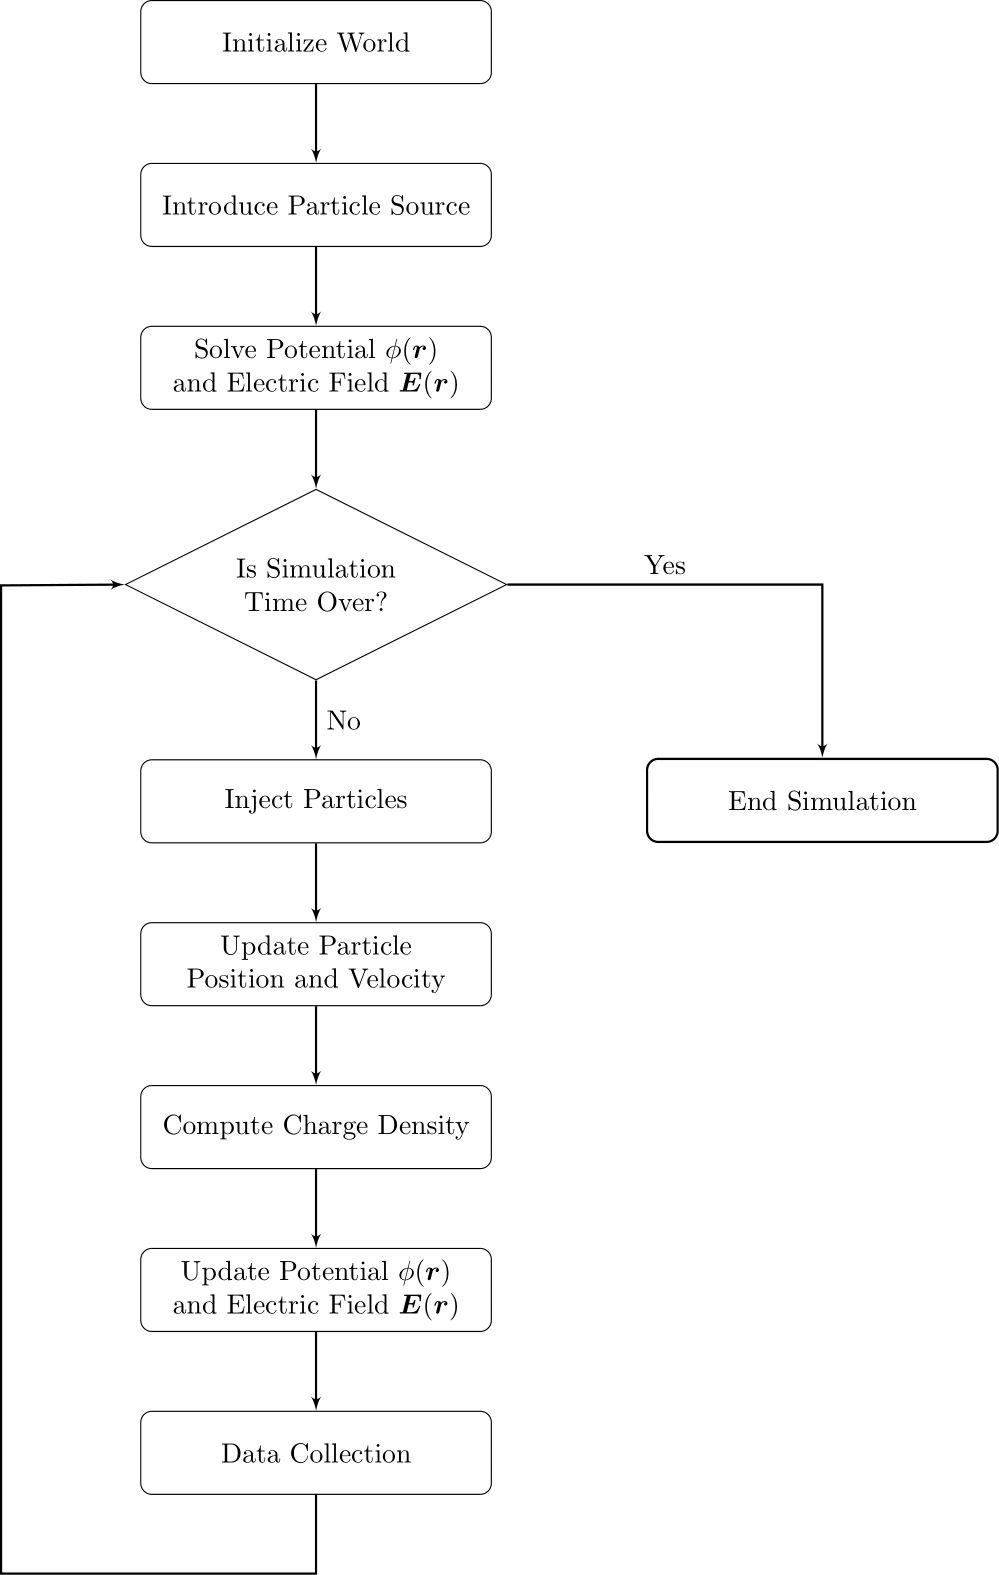
\includegraphics[width=0.7\linewidth]{figures/chapter 2/Flowchart_Studienprojekt-1.png}
    \caption{Caption}
    \label{fig:enter-label}
\end{figure}

\section{Lorentz Force}

\section{Maxwells Equations}

\subsection{Poisson Equation}

\section{Discretize World Domain}

\section{Potential Solver}

\subsection{Gauss Seidel}

\subsection{Seccesive Over Relaxation}

\section{Electric Field Solver}

\section{Particle Motion}

\subsection{Leapfrog Method}

\subsection{Interpolation}

\section{Introduction Particle Sources}

\subsection{Quiet Start method}


\chapter{Implementaion}
\label{Chap: experimenantal part}

\section{Introducing Objects}
\label{Sec: Introducing Objects}

In simulating real-world phenomena, it is essential to incorporate geometric shapes into the simulation environment to represent physical boundaries and objects accurately. The complexity of these shapes can vary significantly depending on the specific problem at hand, and selecting the appropriate coordinate system plays a critical role in simplifying the implementation. However, for ease of integration, a cartesian coordinate system is used throughout the simulations outlined in this report. While the general procedure of implementing geometric shapes in the simulation remains the same, this section exemplifies the process by focusing on two specific three-dimensional shapes. The first is a sphere, which is geometrically defined by its center vector and radius. To simulate the interaction between charged particles and the sphere, all grid nodes located within the sphere are assigned a fixed electric potential. This can be implemented in the simulation using the following approach:

\begin{figure}[H]
    \centering
    \begin{lstlisting}
def add_sphere(self, x0, radius, phi_sphere):
    self.sphere_x0 = Vec3(*x0)  # Save sphere centroid
    self.sphere_rad2 = radius * radius  # Save radius squared
    
    # Loop over all nodes
    for i in range(self.ni):
        for j in range(self.nj):
            for k in range(self.nk):
                x = self.pos(i, j, k)  # Node position
                if self.in_sphere(x):
                    self.objectid.data[i, j, k] = 1  # Set object flag
                    self.phi.data[i, j, k] = phi_sphere  # Set potential

def in_sphere(self, x):
    """Check if a point x is inside the sphere."""
    return (x-self.sphere_x0).dot(x-self.sphere_x0) <= self.sphere_rad2
\end{lstlisting}
    \caption{Caption}
    \label{fig:enter-label}
\end{figure}

The basic procedure involves iterating over all nodes in the system and checking whether each point lies within the desired geometry. If this condition is met, the node is assigned a specific object value, allowing for the storage of information about the simulation world for further analysis in tools such as ParaView. An illustration of such a charged sphere is shown below:

\begin{figure}[H]
    \centering
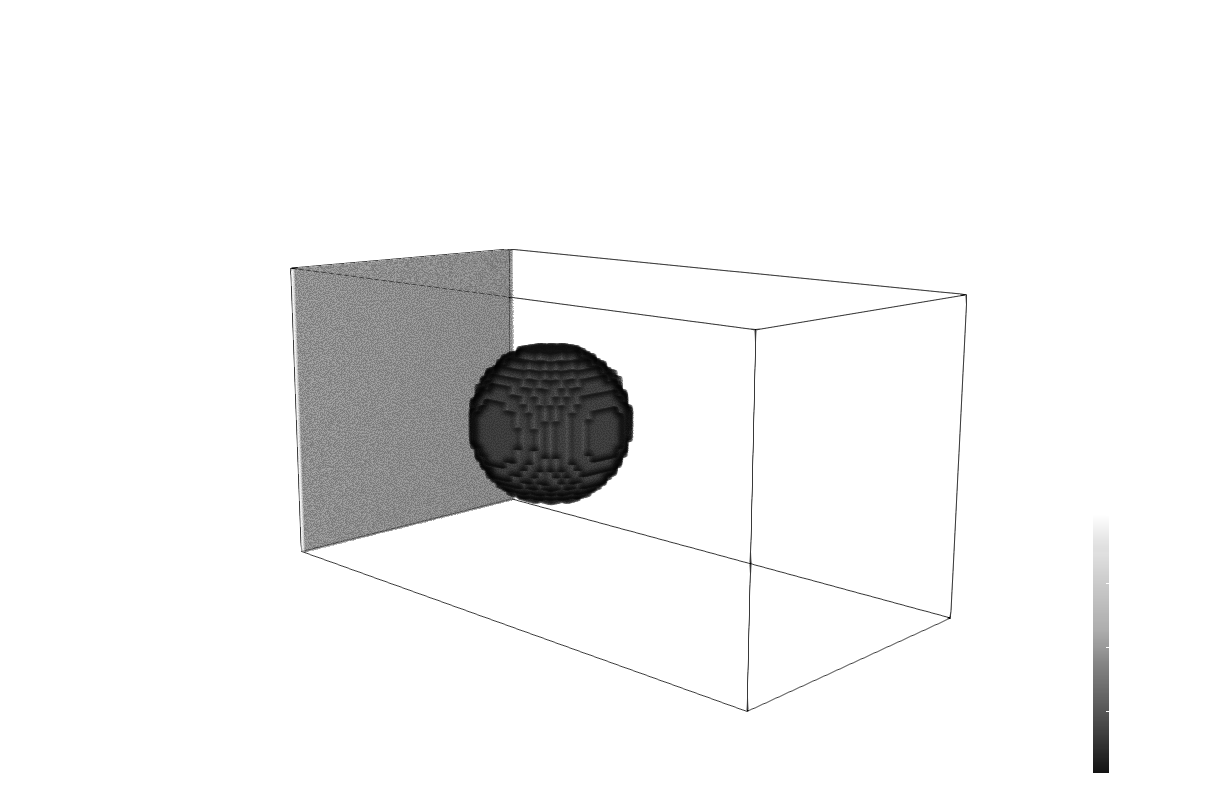
\includegraphics[width=0.7\linewidth]{figures/sphere_paraview.png}    
    \caption{Caption}
    \label{fig: Sphere simulation domain}
\end{figure}

The outlined procedure can be extended to simulate more complex geometries commonly found in practical applications, such as those encountered in gridded electrostatic ion thrusters. In those systems, positively charged ions are accelerated and precisely focused by a series of 2 or 3 grids, each containing typically thousands of coaxial apertures \cite{noauthor_gridded_nodate}. The ions are accelerated due to the potential difference between the first and the second grid, known as the screen and the accelerator grid, respectively \cite{foster_review_2024}. Simulating these ion thrusters accurately requires modeling variations in the thickness and size of the grid structure, as well as the electric potential applied to each grid. A simplistic version of such a grid aperture can be implemented using the following approach:
\begin{figure}[H]
    \centering
    \begin{lstlisting}
def add_plane_with_hole(self, z_0, thickness, phi_plane, hole_0,hole_r):

# Loop over all nodes
for i in range(self.ni):
    for j in range(self.nj):
        for k in range(self.nk):
            x, y, z = self.pos(i, j, k)  # coordinates of the current node
            
            # Calculate the distance from the hole-center in the XY plane
            xy_dist2 = (x - hole_0[0]) ** 2 + (y - hole_0[1]) ** 2
            
            # Check if the current node is within the plane thickness
            # and outside the circular hole area
            if z_0 <= z < (z_0 + thickness) and xy_dist2 > hole_radius2:
                self.objectid.data[i, j, k] = 1  # Set object flag
                self.phi.data[i, j, k] = phi_plane  # Set potential
    \end{lstlisting}
    \caption{Caption}
    \label{fig:enter-label}
\end{figure}

Such a system can be effectively visualized using ParaView, providing a detailed representation of the grid structure and particle dynamics. The following illustration demonstrates two grids with apertures of varying plane thickness and size. On the left side of the simulation domain is an inlet, from which charged particles could be injected at a specified drift velocity:
\begin{figure}[H]
    \centering
    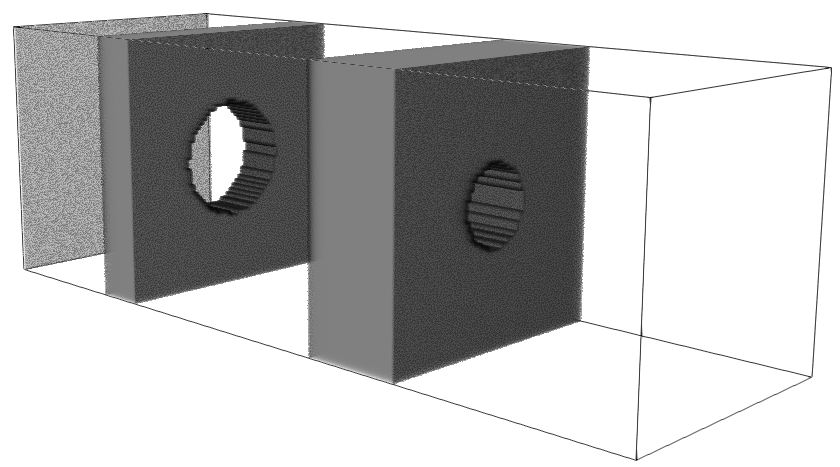
\includegraphics[width=0.7\linewidth]{figures/GIT_Paraview.png}
    \caption{Caption}
    \label{fig:enter-label}
\end{figure}
\section{Optimizing of the Relaxation Factor}
\label{Sec: Optimizing Relaxation Factor}

\usepackage{graphicx}   % For including graphics
\usepackage{subcaption} % For subfigures

\begin{figure}[H]
    \centering
    \begin{subfigure}[b]{0.55\linewidth}
        \centering
        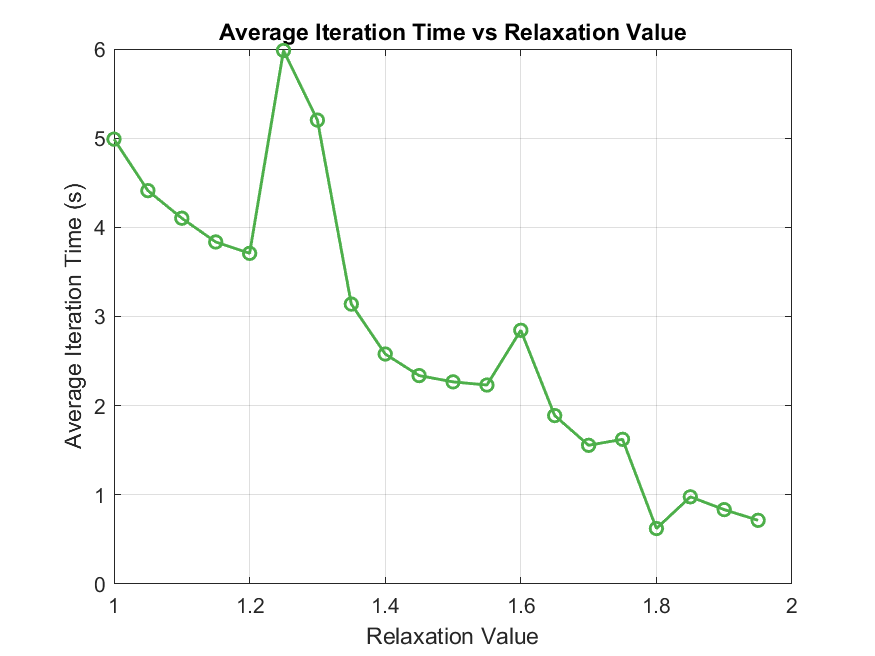
\includegraphics[width=\linewidth]{figures/overrelaxation/average_iteration_time_vs_relaxation_value.png}
        \caption{Average Iteration Time vs Relaxation Value}
        \label{fig:average_iteration_time}
    \end{subfigure}
    \hfill
    \begin{subfigure}[b]{0.55\linewidth}
        \centering
        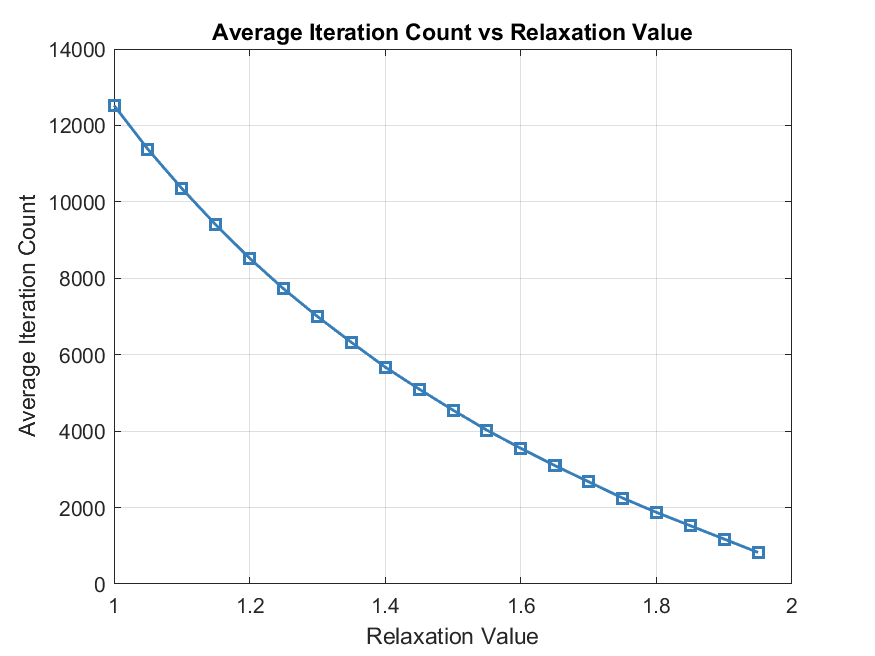
\includegraphics[width=\linewidth]{figures/overrelaxation/average_iteration_count_vs_relaxation_value.png}
        \caption{Average Iteration Count vs Relaxation Value}
        \label{fig:average_iteration_count}
    \end{subfigure}
    \caption{Comparison of Average Iteration Time and Count with Relaxation Values}
    \label{fig:comparison}
\end{figure}

\section{Simulation Outcomes}\label{Sec: Simulation Outcomes}

This section presents the simulation outcomes for two specific cases: the flow of charged particles around a sphere and the behavior of ions in a grid potential layout similar to those found in gridded electrostatic ion thrusters. These simulations are evaluated by examining energy conservation within the system, serving as a key indicator to verify the plausibility of the results. Furthermore, the steady state of the simulation is introduced, where key properties of the system, such as mass, momentum, energy, and charge, become time-invariant. This condition defines the point at which further iterations no longer provide significant changes to the results, indicating the simulation has reached equilibrium. Lastly, the limitations of the current implementation of the electrostatic particle-in-cell (\acs{ES PIC}) method are outlined and demonstrated through a specific challenge encountered during simulation.

\subsection{Flow Around a Sphere}\label{Sec: Flow Around Sphere}

In this section, a sphere with a fixed potential of $\Phi = -100V$ is introduced within the simulation domain, as illustrated in Fig. \ref{fig: Sphere simulation domain}. Oxygen ions (O+) with a single positive charge are injected from the inlet on the left plane, maintaining a particle density of \SI{1e10}{\per\meter^3} and a drift velocity of 7000 m/s. The sphere serves as a particle sink, absorbing ions upon interaction. As a result, a condensed stream forms behind the sphere, characterized by a region of increased ion density. This phenomenon arises due to the lensing effect, where the sphere deflects ion trajectories, concentrating them in the region downstream \cite{brieda_plasma_2019}.

\begin{figure}[H]
    \centering
    \begin{subfigure}[b]{0.49\linewidth}
        \centering
        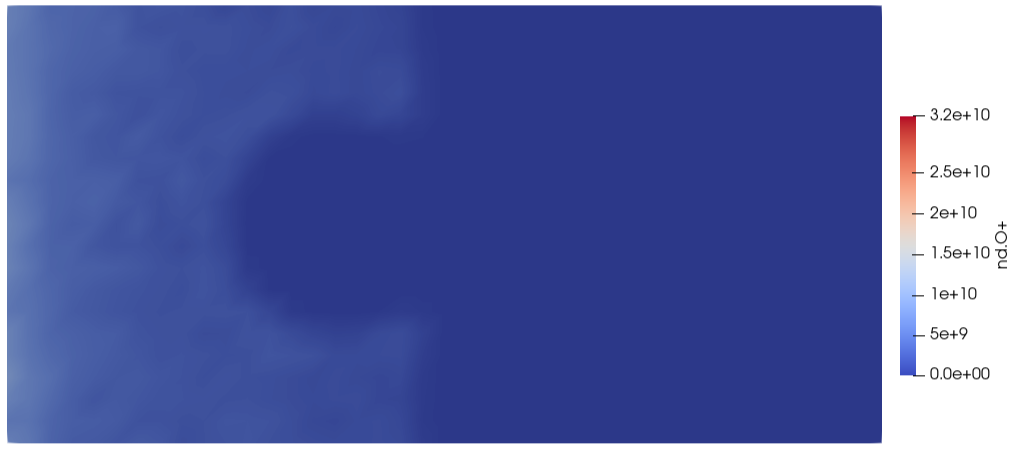
\includegraphics[width=\linewidth]{figures/Sphere/80_iterations.png}
        \caption{80 Iterations}
        \label{fig:average_iteration_time}
    \end{subfigure}
    \hfill
    \begin{subfigure}[b]{0.49\linewidth}
        \centering
        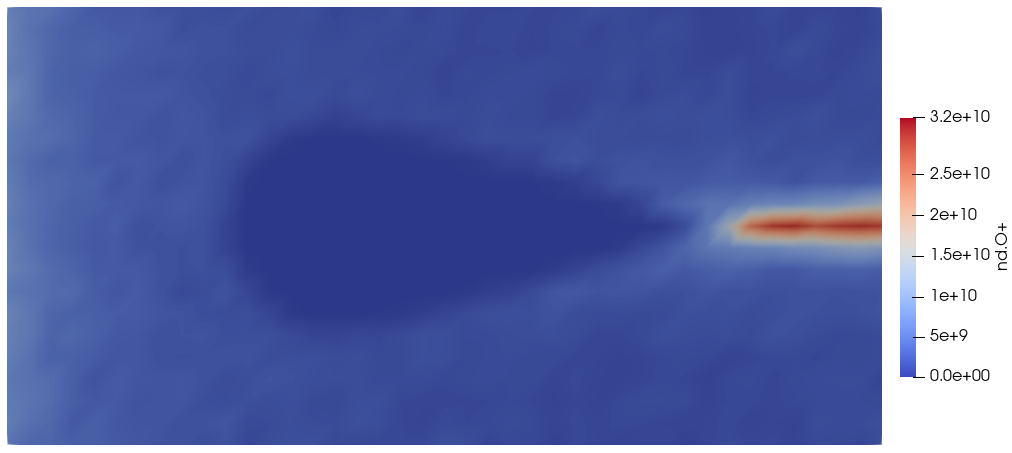
\includegraphics[width=\linewidth]{figures/Sphere/160_iterations.png}
        \caption{160 Iterations}
        \label{fig:average_iteration_count}
    \end{subfigure}
    \caption{Comparison of Average Iteration Time and Count with Relaxation Values}
    \label{fig:comparison}
\end{figure}


steady state 

only changes through noise introduced by the randomized injection of particles!

Therefore some fluctuations


\begin{figure}[H]
    \centering
    \begin{subfigure}[b]{0.49\linewidth}
        \centering
        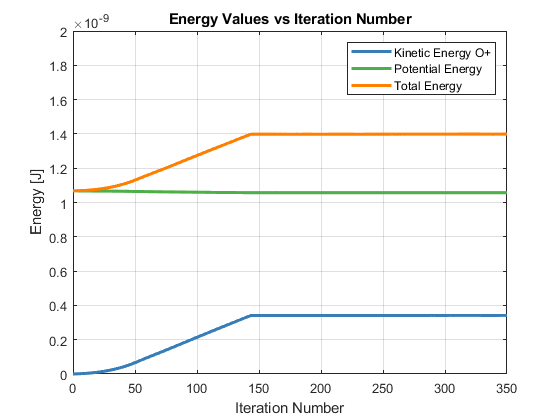
\includegraphics[width=\linewidth]{figures/Sphere/energy_values_plot.png}
        \caption{Energy}
        \label{fig:average_iteration_time}
    \end{subfigure}
    \hfill
    \begin{subfigure}[b]{0.49\linewidth}
        \centering
        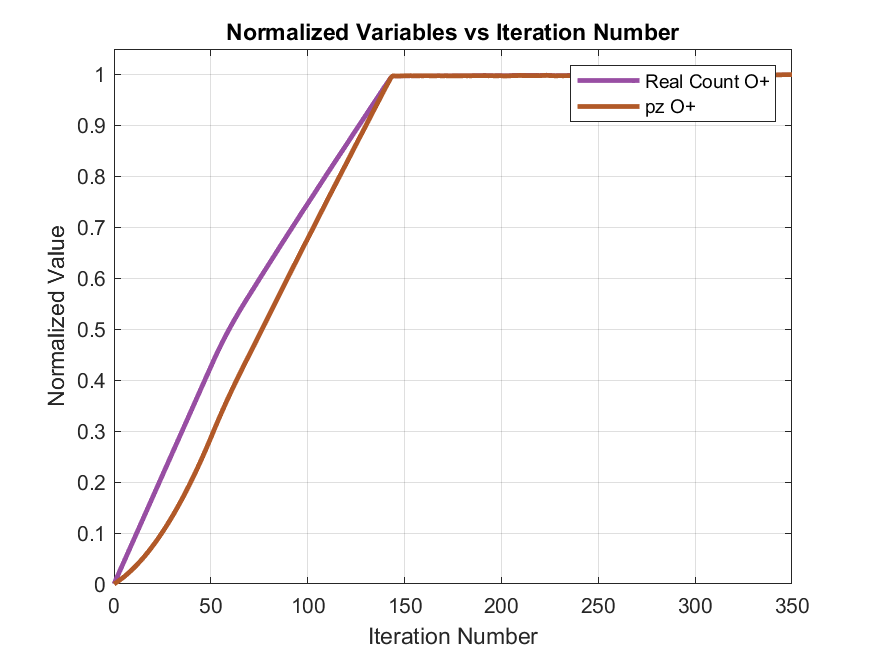
\includegraphics[width=\linewidth]{figures/Sphere/normalized_variables_plot.png}
        \caption{other variables}
        \label{fig:average_iteration_count}
    \end{subfigure}
    \caption{Comparison of Average Iteration Time and Count with Relaxation Values}
    \label{fig:comparison}
\end{figure}

Expected results the potential energy resulting from the grids remains constant in the system

however the kinetic energy and therefore the the total energy in the system increases until the steady state is achieved.

This happens after roughly 145 iterations at which point the total amount of particles in the system remains the same.

Those outcomes are consistent with the results presented for a similar simulation outlined in \cite{brieda_plasma_2019}.

\subsection{Basic Framework for Grid Potential Layout in RIT Thruster Design}
\section{Discussion}\label{Sec: Discussion}

\chapter{Future Work}
\chapter{Conclusion}
% Hier wird das Literaturverzeichnis eingebunden
%\printbibliography


\printbibliography[title={Bibliography}, heading=bibintoc]

\cleardoublepage

\appendix

%\chapter{Ergänzende Informationen 1}
%\blindtext


\end{document} 